\documentclass[aspectratio=169]{beamer}
\usepackage[utf8]{inputenc}
\usepackage[T1]{fontenc}
\usepackage{tikz}

\usetheme{Singapore}

\hypersetup{pdfstartview={Fit}}

\title{Fusionsreaktoren (Konzepte)}
\subtitle{}
\author{Leon Schwarzer und Emile Hansmaennel}
\institute{Theodor-Fliedner-Gymnasium}
\date{\today}


\begin{document}
  \begin{frame}
    \titlepage
  \end{frame}

  \section{Allgemeines}
    \subsection{Titel}

      \begin{frame}
        \frametitle{Was ist ein Fusionsreaktor?}
        Ein \textbf{Kernfusionsreaktor} oder \textbf{Fusionsreaktor} ist eine
        technische Anlage, in der die \textbf{Kernfusion} von Deuterium und Tritium als
        \textbf{thermonukleare Reaktion} kontrolliert abläuft.
        \par
        \raggedleft
        Wikipedia - Kernfusionsreaktor
      \end{frame}

      \begin{frame}
        \frametitle{Warum nutzen wir keine Fusionsreaktoren?}
        \center
        Zu viel Energie rein \( \rightarrow \) zu wenig Energie raus
      \end{frame}

    \subsection{Arten}

      \begin{frame}
        \frametitle{Arten von Fusionsreaktoren}
        \begin{columns}
          \column{0.5\textwidth}
          \center
          Stellatoren \( \rightarrow \) USA

          \begin{figure}
            \centering
            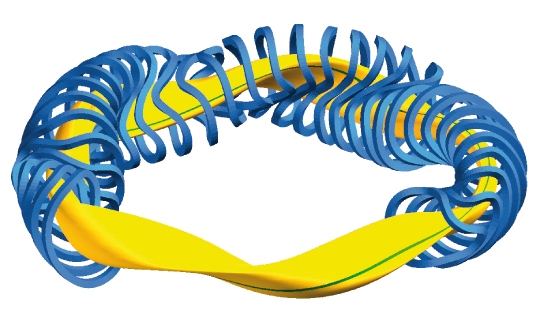
\includegraphics[width=0.5\textwidth]{figs/stellator}
            \caption{Schematische Darstellung}
            \label{figure:stellator}
          \end{figure}
          \begin{figure}
            \centering
            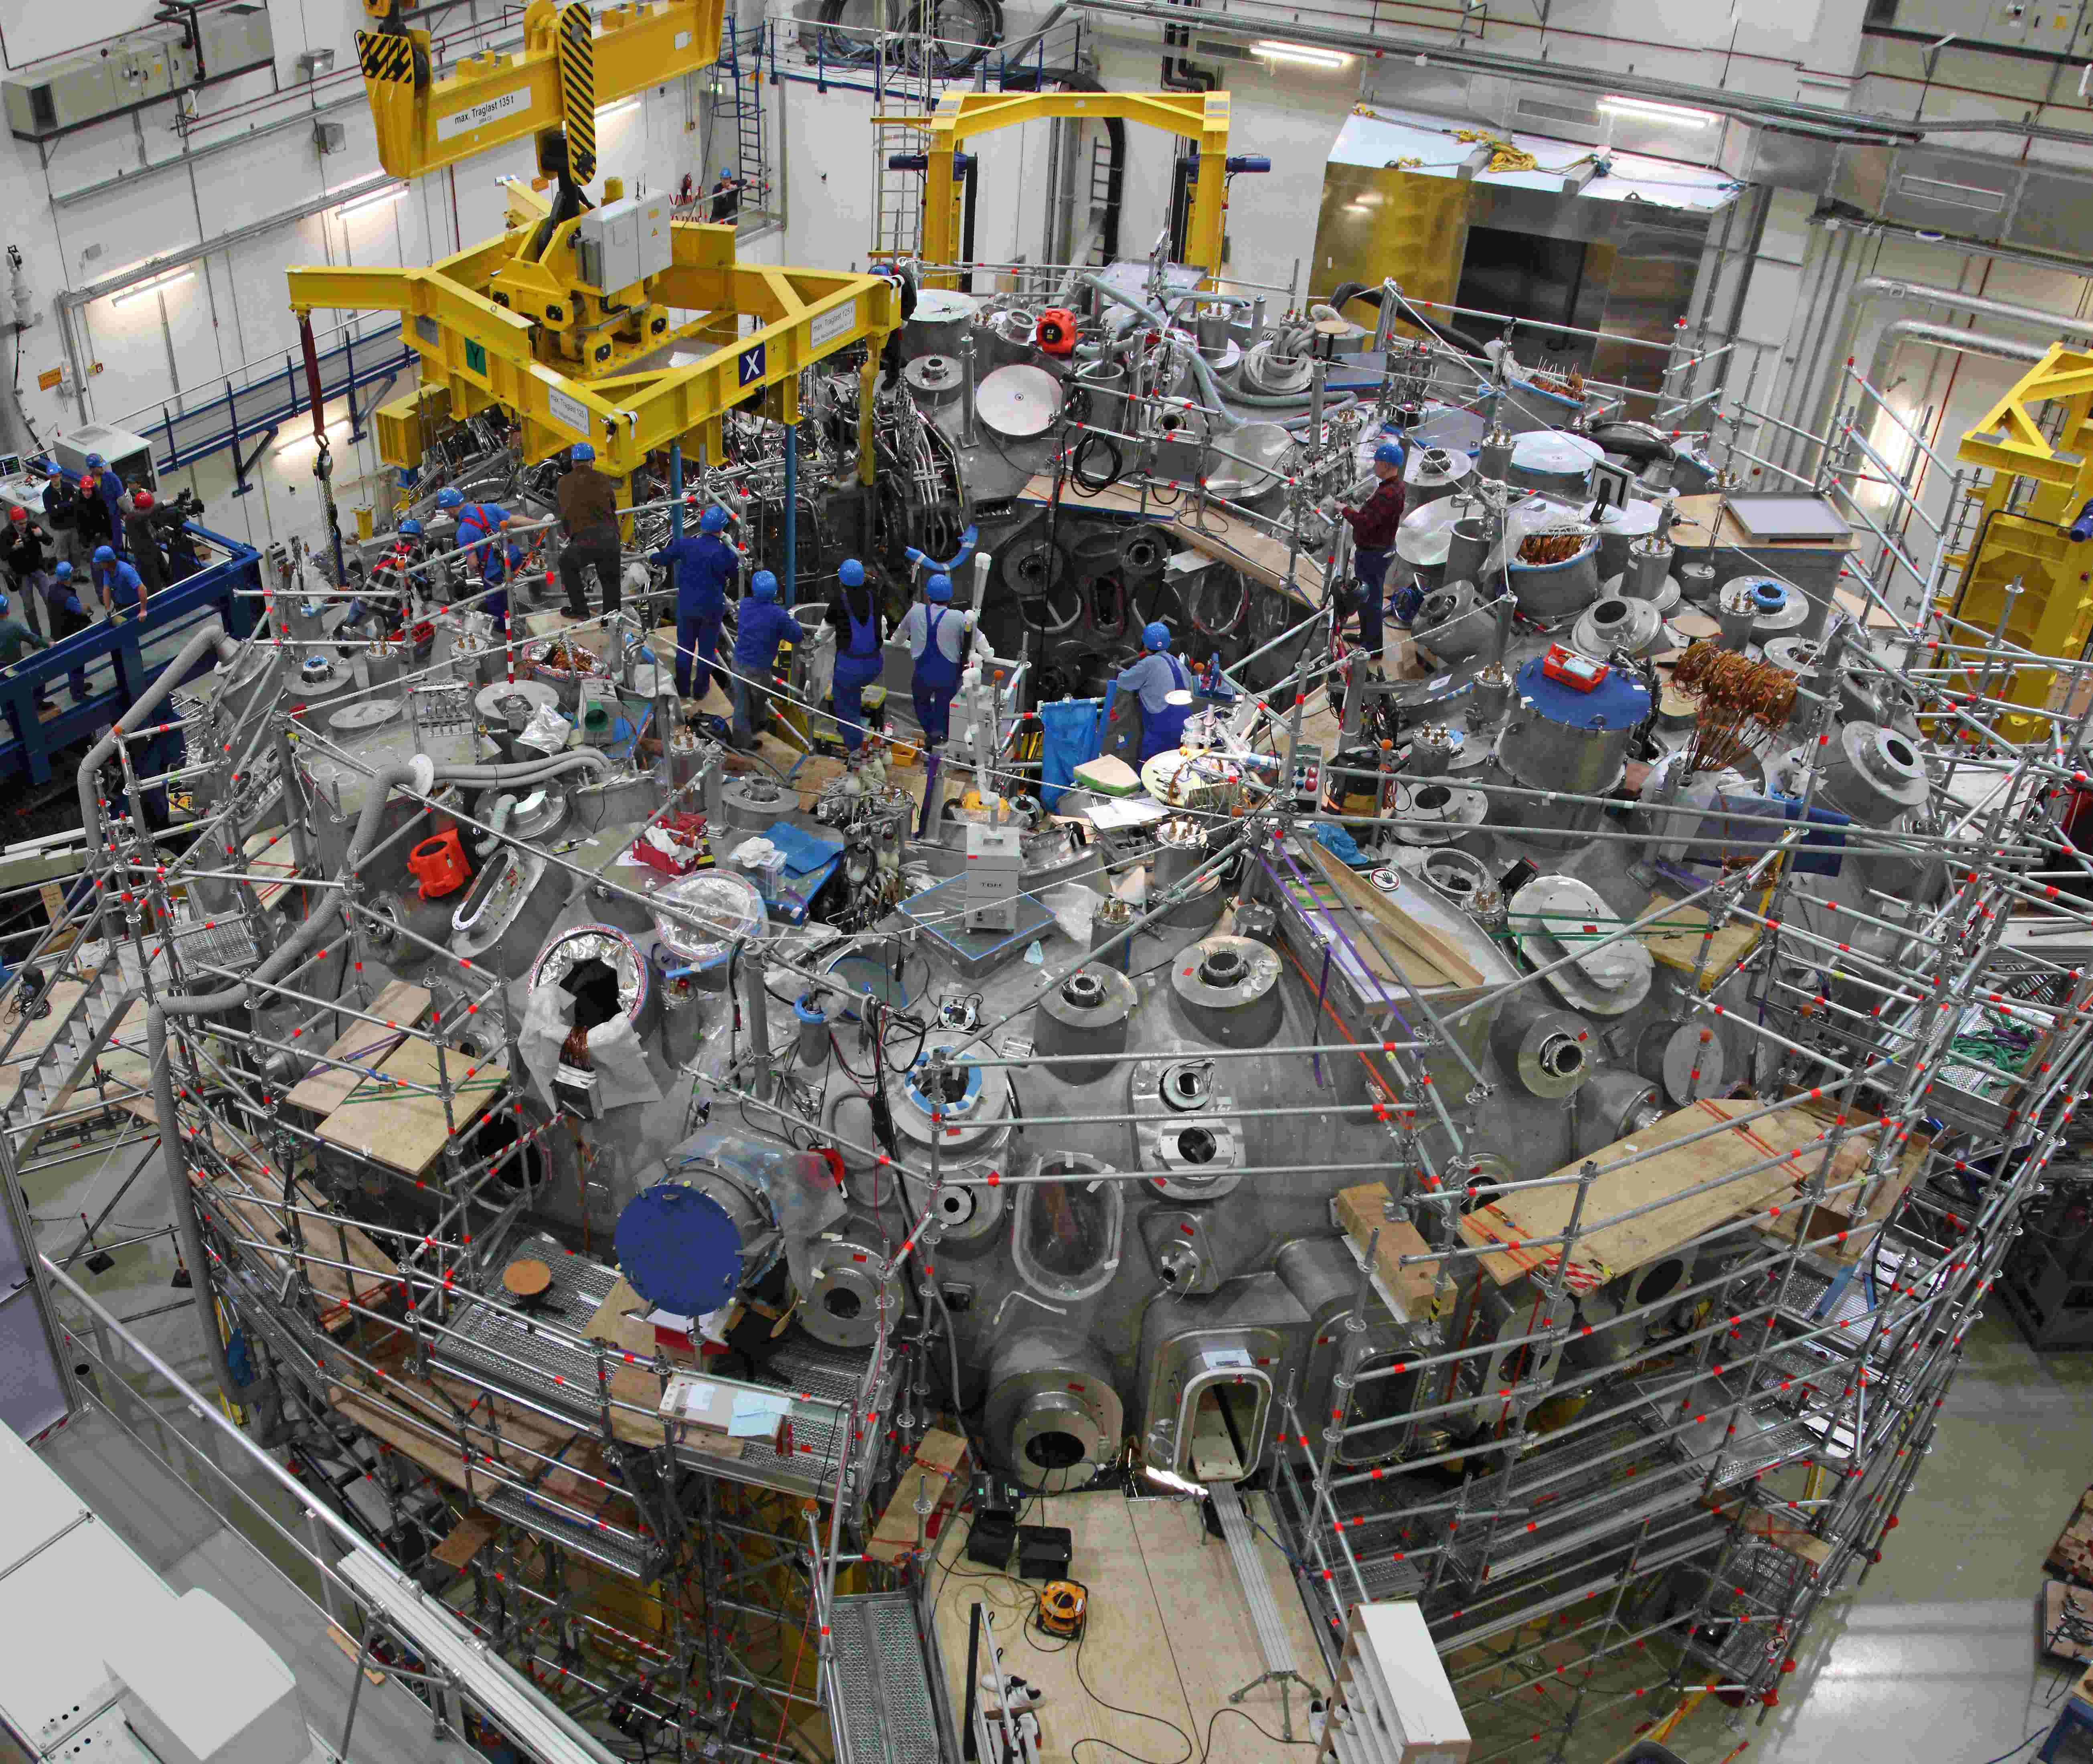
\includegraphics[width=0.5\textwidth]{figs/wendelstein}
            \caption{Wendelstein 7-X Ende 2011}
            \label{figure:stellator}
          \end{figure}

          \bigskip
          \column{0.5\textwidth}
          \center
          Tokamaks \( \rightarrow \) Sowiet-Union

          \begin{figure}
            \centering
            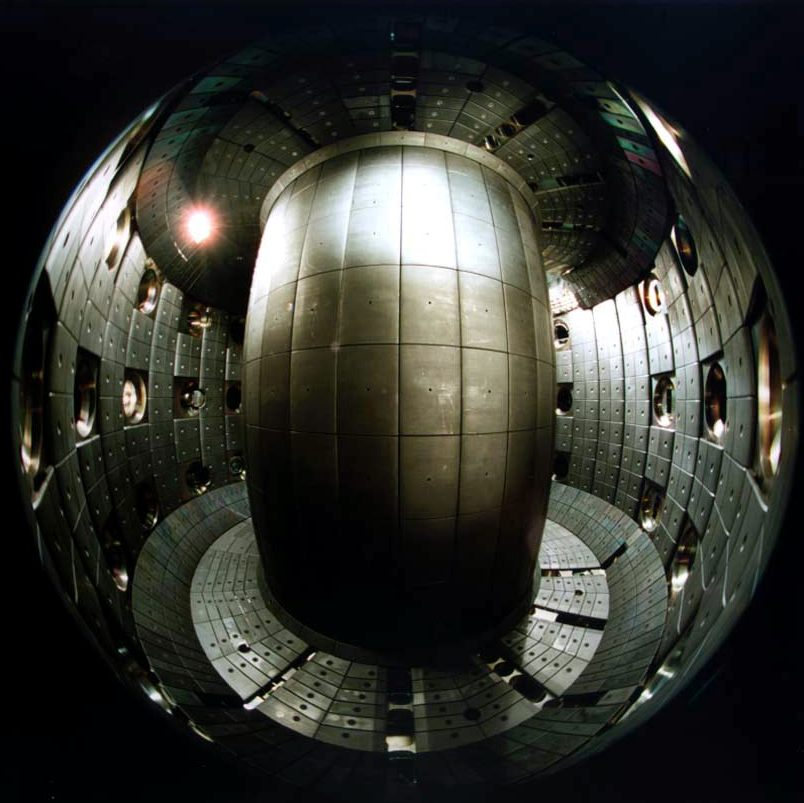
\includegraphics[width=0.5\textwidth]{figs/tokamak_innen}
            \caption{Innenraum des mit Graphitplatten ausgekleideten Tokamak à configuration variable (TCV) in Lausanne, Schweiz}
            \label{figure:tokamak_innen}
          \end{figure}

        \end{columns}
      \end{frame}

      \begin{frame}
        \frametitle{Stellatoren}
      \end{frame}

      \begin{frame}
        \frametitle{Tokamaks}
      \end{frame}

  \section{Physikalische Grundlagen}

    \subsection{Was Passiert?}

      \begin{frame}
        \frametitle{Was passiert bei der Kernfusion?}
        \center
        Kernfusion von Deuterium und Tritium als thermonukleare Reaktion:

        \bigskip
        \pause
        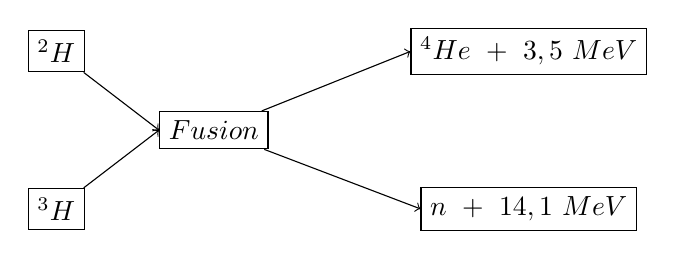
\begin{tikzpicture}
        \node[draw] at (0, 0) (2H) { \( {}^2H \) };
        \node[draw] at (0, -2) (3H) { \( {}^3H \) };
        \node[draw] at (2, -1) (fusion) { \( Fusion \) };
        \node[draw] at (6, 0) (4He) { \( {}^4He~+~3,5~MeV \) };
        \node[draw] at (6, -2) (n) { \( n~+~14,1~MeV \) };

        \draw[->] (2H) edge (fusion.west);
        \draw[->] (3H) edge (fusion.west);
        \draw[->] (fusion) -- (4He.west);
        \draw[->] (fusion) -- (n.west);

        \end{tikzpicture}

        \bigskip

        Ein \textbf{Deuterium}- und ein \textbf{Tritium}-Atomkern verschmelzen zu einem \textbf{Heliumkern} unter Freisetzung eines \textbf{schnellen Neutrons}.

      \end{frame}

    \subsection{Reaktion}

      \begin{frame}
        \frametitle{Deuterium-Tritium-Reaktion}
        \begin{itemize}
          \item Atomkerne verschmelzen zu einem neuem Kern
          \item Energie wird freigesetzt
          \item Atomkerne kommen sich sehr nahe (2,5 Femtometer)
          \item Masse Vorher \( > \) Masse Nachher \( \rightarrow \) Differenz wird zu Energie
        \end{itemize}
        \bigskip

        \begin{columns}[T]
          \begin{column}{0.5\textwidth}
            \begin{equation*}
              D + T \rightarrow {}^4 H + n + \underbrace{ 17,6~MeV }_{Gewonnene~Energie}
            \end{equation*}
          \end{column}
          \begin{column}{0.5\textwidth}
            \begin{equation*}
              E = mc^2
            \end{equation*}
          \end{column}
        \end{columns}
      \end{frame}

  % \section{Technik}
  %   \subsection{Allgemein}
  %
  %     \begin{frame}
  %       \frametitle{Fusion mit magnetischem Plasmaeinschluss}
  %       Lorem ipsum dolor sit amet, consectetur adipisicing elit, sed do eiusmod tempor incididunt ut labore et dolore magna aliqua. Ut enim ad minim veniam, quis nostrud exercitation ullamco laboris nisi ut aliquip ex ea commodo consequat. Duis aute irure dolor in reprehenderit in voluptate velit esse cillum dolore eu fugiat nulla pariatur. Excepteur sint occaecat cupidatat non proident, sunt in culpa qui officia deserunt mollit anim id est laborum.
  %     \end{frame}
  %
  %   \subsection{Plasmaaufheizung}
  %
  %     \begin{frame}
  %       \frametitle{Plasmaaufheizung}
  %       \begin{itemize}
  %         \item Ziel: Plasma auf über 1000 grad Celsius aufzuheizen
  %         \pause
  %         \item Achtung: (Deuteriumkerne haben bei 100 Mio. C eine mittlere
  %         Geschwindigkeit von etwa 1000 km/s)
  %       \end{itemize}
  %     \end{frame}
  %
  %     \begin{frame}
  %       \frametitle{Plasmaaufheizung}
  %       \framesubtitle{\underline{Elektrisches Aufheizen}}
  %       Das Plasma ist ein elektrischer Leiter und kann mittels eines induzierten elektrischen Stroms aufgeheizt werden. Dabei ist das Plasma die Sekundärspule eines Transformators. Allerdings steigt die Leitfähigkeit des Plasmas mit steigender Temperatur, so dass der elektrische Widerstand ab etwa 20–30 Millionen Grad bzw. 2 keV nicht mehr ausreicht, das Plasma stärker zu erhitzen.
  %     \end{frame}
  %
  %     \begin{frame}
  %       \frametitle{Plasmaaufheizung}
  %       \framesubtitle{\underline{Neutralteilchen-Einschuss}}
  %       Beim Einschießen schneller neutraler Atome in das Plasma (neutral beam injection, kurz NBI) wird die kinetische Energie dieser Atome – die im Plasma sofort ionisiert werden – durch Stöße auf das Plasma übertragen, wodurch sich dieses aufheizt.
  %     \end{frame}
  %
  %     \begin{frame}
  %       \frametitle{Plasmaaufheizung}
  %       \framesubtitle{\underline{Elektromagnetische Wellen}}
  %       Mikrowellen können die Ionen und Elektronen im Plasma auf ihren Resonanzfrequenzen (Umlauffrequenz in der Schraubenlinie, die das Teilchen im Magnetfeld beschreibt) anregen und somit Energie in das Plasma übertragen. Diese Methoden des Aufheizens werden Ion Cyclotron Resonance Heating (ICRH), Electron Cyclotron Resonance Heating (ECRH) und Lower Hybrid Resonance Heating (LHRH) genannt.
  %     \end{frame}
  %
  %     \begin{frame}
  %       \frametitle{Plasmaaufheizung}
  %       \framesubtitle{Magnetische Kompression}
  %       Das Plasma kann wie ein Gas durch schnelles (adiabatisches) Zusammenpressen erwärmt werden. Ein zusätzlicher Vorteil dieser Methode ist, dass zugleich die Plasmadichte erhöht wird. Nur von Magnetspulen mit veränderbarer Stromstärke erzeugte Magnetfelder sind geeignet, das Plasma zusammen zu pressen; von supraleitenden Magnetspulen erzeugte Magnetfelder sind dafür nicht geeignet, weil ihre Stärke unveränderlich ist.
  %     \end{frame}
  %
  %   \subsection{Magnetfeld}
  %
  %     \begin{frame}
  %       \frametitle{Magnetfeld}
  %       \begin{itemize}
  %         \item Hält das Plasma zusammen, damit es nicht die Gefäßwand berührt
  %         \( \rightarrow \) Torusförmiges, verdrilltes Magnetfeld
  %         \item Besondere Verformungen entfernen die unerwünschten Ionen und andere Verunreinigungen
  %
  %       \end{itemize}
  %     \end{frame}
  %
  % \section{Brennstoff}
  %   \subsection{Vorkommen / Beschaffung}
  %
  %     \begin{frame}
  %       \frametitle{Vorkommen und Beschaffung}
  %
  %       Auf der Erde gibt es:\\
  %
  %       \( \approx 2,5 \cdot 10^{13}\) Tonnen Deuterium \( \rightarrow \) genug
  %       ,aber kein Tritium!
  %
  %       Es wird \( {}^6Li\) genutzt, dass in Tritium umgewandelt wird:
  %
  %       \begin{equation}
  %         {}^6Li + n \rightarrow {}^4He + {}^3H+ 4,8MeV
  %       \end{equation}
  %
  %     \end{frame}
  %
  %     \begin{frame}
  %       \frametitle{Tritiumbrüten und Neutronenvermehrung}
  %       Lorem ipsum dolor sit amet, consectetur adipisicing elit, sed do eiusmod tempor incididunt ut labore et dolore magna aliqua. Ut enim ad minim veniam, quis nostrud exercitation ullamco laboris nisi ut aliquip ex ea commodo consequat. Duis aute irure dolor in reprehenderit in voluptate velit esse cillum dolore eu fugiat nulla pariatur. Excepteur sint occaecat cupidatat non proident, sunt in culpa qui officia deserunt mollit anim id est laborum.
  %     \end{frame}
  %
  %   \subsection{Brennstoffnachfüllung}
  %
  %     \begin{frame}
  %       \frametitle{Brennstoffnachfüllung}
  %       Lorem ipsum dolor sit amet, consectetur adipisicing elit, sed do eiusmod tempor incididunt ut labore et dolore magna aliqua. Ut enim ad minim veniam, quis nostrud exercitation ullamco laboris nisi ut aliquip ex ea commodo consequat. Duis aute irure dolor in reprehenderit in voluptate velit esse cillum dolore eu fugiat nulla pariatur. Excepteur sint occaecat cupidatat non proident, sunt in culpa qui officia deserunt mollit anim id est laborum.
  %     \end{frame}
  %
  %   \subsection{Entfernen von Verunreinigungen}
  %
  %     \begin{frame}
  %       \frametitle{Entfernen von Helium und Verunreinigungen}
  %       Lorem ipsum dolor sit amet, consectetur adipisicing elit, sed do eiusmod tempor incididunt ut labore et dolore magna aliqua. Ut enim ad minim veniam, quis nostrud exercitation ullamco laboris nisi ut aliquip ex ea commodo consequat. Duis aute irure dolor in reprehenderit in voluptate velit esse cillum dolore eu fugiat nulla pariatur. Excepteur sint occaecat cupidatat non proident, sunt in culpa qui officia deserunt mollit anim id est laborum.
  %     \end{frame}

  % \section{Bau eines Reaktors}
  %
  %   \begin{frame}
  %     \frametitle{Materialien / Chemikalien}
  %     \begin{itemize}
  %       \item \( {}^2H, {}^3H, Fe, ... \)
  %     \end{itemize}
  %   \end{frame}
  %
  %   \begin{frame}
  %     \frametitle{Beispiel: ITER (Süd Frankreich)}
  %     \center
  %     \textbf{50} Mega Watt Input \( \rightarrow \) \textbf{500} Mega Watt Output
  %   \end{frame}

  \section{Stand der Forschung}

    \begin{frame}
      \frametitle{Wo sind wir zurzeit???}

      Die drei entscheidenden Größen ( \textbf{Temperatur} \( T \), \textbf{Teilchendichte} \( n_e \)
      und \textbf{Energieeinschlusszeit} \( \tau_E \) ) wurden in den letzten 50 Jahren
      erheblich vergrößert und das \textbf{Tripelprodukt} \( T \cdot n_e \cdot \tau_E \)
      etwa um den Faktor 10.000 verbessert.

    \end{frame}

  \section{Quellen / Weiteres}

    \begin{frame}
      \frametitle{Quellen}
      \begin{itemize}
        \item https://de.wikipedia.org/wiki/Kernfusionsreaktor
        \item https://www.iter.org/proj/inafewlines
      \end{itemize}
    \end{frame}

\end{document}
